%========================================================================
% Chapter 4: Implementation and Discussion
%========================================================================
\chapter{Implementation and Discussion}

\section{Methodology}

NepTube was developed following a systematic approach \cite{schwaber2020scrum}, beginning with requirement analysis to identify essential features such as user authentication, video uploading, AI-powered recommendations, premium subscription management, and creator analytics. The project utilizes Next.js \cite{vercel2024nextjs} with TypeScript \cite{typescript2024docs} for both frontend and backend development, ensuring a unified and scalable codebase. Drizzle ORM \cite{drizzle2024docs} was chosen for database management, while Clerk \cite{clerk2024docs} handles authentication and UploadThing \cite{uploadthing2024docs} manages file uploads.

The development process followed modular architecture principles, starting with implementing user registration and authentication, then building video upload and streaming functionalities. AI integration was achieved using Pollinations \cite{pollinations2024api} and HuggingFace APIs for content analysis, thumbnail generation, and moderation \cite{risch2020toxic}. Premium features were gated using tier management logic, and creator dashboards were developed to provide real-time analytics and monetization predictions. Testing was performed at each stage to ensure reliability across browsers and devices. Deployment was streamlined using Vercel for hosting and automatic scaling, making the development cycle efficient and manageable.

\section{Implementation Steps}

\begin{enumerate}[leftmargin=2cm]
  \item \textbf{Requirement Analysis:} Identified core features including user authentication, video uploading, AI-powered recommendations, premium subscriptions, and creator analytics.

  \item \textbf{Project Setup:} Initialized the Next.js project with TypeScript, configured Drizzle ORM for database management, and integrated Clerk for authentication.

  \item \textbf{Video Upload Module:} Developed video upload functionality using UploadThing, allowing creators to upload and manage content.

  \item \textbf{AI Integration:} Connected Pollinations \cite{pollinations2024api} and Replicate \cite{replicate2024whisper} APIs for thumbnail generation, content analysis, transcription via Whisper~v3 \cite{radford2023whisper}, and content moderation.

  \item \textbf{Premium Features:} Implemented tier management logic with payment integration through eSewa \cite{esewa2024}, Khalti \cite{khalti2024}, Stripe, and PayPal to gate premium features and subscription access.

  \item \textbf{Creator Dashboard:} Built dashboards for creators to view analytics, monetization predictions, and engagement metrics.

  \item \textbf{Testing:} Conducted unit and end-to-end tests to ensure reliability and compatibility.
\end{enumerate}

\section{Output Obtained}

\subsection{Admin Features}
\begin{itemize}[leftmargin=2cm]
  \item Access to an admin dashboard for monitoring platform activity and analytics.
  \item Ability to moderate content, manage user accounts, and review flagged videos or comments.
  \item Tools for overseeing premium subscriptions and resolving disputes.
  \item Real-time insights into platform performance and user engagement.
\end{itemize}

\subsection{Creator Features}
\begin{itemize}[leftmargin=2cm]
  \item Secure registration and authentication via Clerk.
  \item Upload videos and generate AI-powered thumbnails using UploadThing and Pollinations API.
  \item Access to creator dashboards with analytics, monetization predictions, and engagement metrics.
  \item Ability to manage playlists, interact with viewers, and utilize premium features.
  \item Receive feedback on content quality and moderation status.
\end{itemize}

\subsection{User Features}
\begin{itemize}[leftmargin=2cm]
  \item Register and log in securely to the platform.
  \item Browse and watch videos with personalized AI recommendations \cite{covington2016deep, he2017neural}.
  \item Participate in community features such as comments, polls, and Super Chat.
  \item Access premium features based on subscription tier, including downloads and advanced analytics.
  \item Experience safe browsing with AI-powered content moderation \cite{risch2020toxic}.
  \item Enjoy adaptive bitrate streaming for smooth playback \cite{flowplayer2023abr, choi2023qoe}.
\end{itemize}

\section{Test Cases}

For implementation of our project, we have done with some special tests such as white box testing and black box testing. White box testing is testing of the internal working or code of software application. Black box testing is system testing from perspective of user or we can say external working.

{\small
\renewcommand{\arraystretch}{1.35}
\begin{longtable}{|c|J{2.4cm}|J{3.0cm}|J{2.8cm}|J{3.0cm}|c|}
\caption{Test Case Table} \label{tab:test-cases} \\
\hline
\textbf{ID} & \textbf{Test Case} & \textbf{Test Steps} & \textbf{Test Data} & \textbf{Expected Result} & \textbf{Status} \\
\hline
\endfirsthead
\hline
\textbf{ID} & \textbf{Test Case} & \textbf{Test Steps} & \textbf{Test Data} & \textbf{Expected Result} & \textbf{Status} \\
\hline
\endhead
\hline
\endfoot
1 & User login with valid data & Navigate to sign-in page and confirm the SignIn form & Email: test1@gmail.com, password: test123 & User should be able to sign in to the system & Pass \\
\hline
2 & User registration with valid data & Navigate to sign-up page and confirm the SignUp form & Email: test2@gmail.com, Password: test123 & User should be able to sign up to the system & Pass \\
\hline
3 & Video upload by creator & Login as creator, navigate to upload page, upload a valid video file & Video file (mp4), Title, Description & Video should be uploaded and visible in creator dashboard & Pass \\
\hline
4 & AI thumbnail generation & Upload a video and request AI-generated thumbnail & Video file (mp4) & AI-generated thumbnail should be displayed & Pass \\
\hline
5 & Comment moderation & Post a comment containing offensive words & ``This is a bad-word comment'' & Comment should be flagged or blocked by moderation system & Pass \\
\hline
6 & Premium feature access & Subscribe to premium and try to access exclusive features & Valid user, active premium subscription & User should access premium features (e.g., downloads, analytics) & Pass \\
\hline
7 & Playlist creation & User creates a new playlist and adds videos & Valid user, video list & Playlist should be created and videos added successfully & Pass \\
\hline
8 & Logout functionality & User clicks logout button & Logged-in user & User should be logged out and redirected to login page & Pass \\
\hline
\end{longtable}
}

\section{Application Screenshots}

This section presents screenshots of the NepTube platform demonstrating the key features and user interfaces implemented during development.

\subsection{Home Page and Video Browsing}

The home page displays a curated grid of video thumbnails with titles, view counts, and creator information. The responsive layout adapts to different screen sizes and supports infinite scrolling for seamless content discovery.

\begin{figure}[H]
\centering
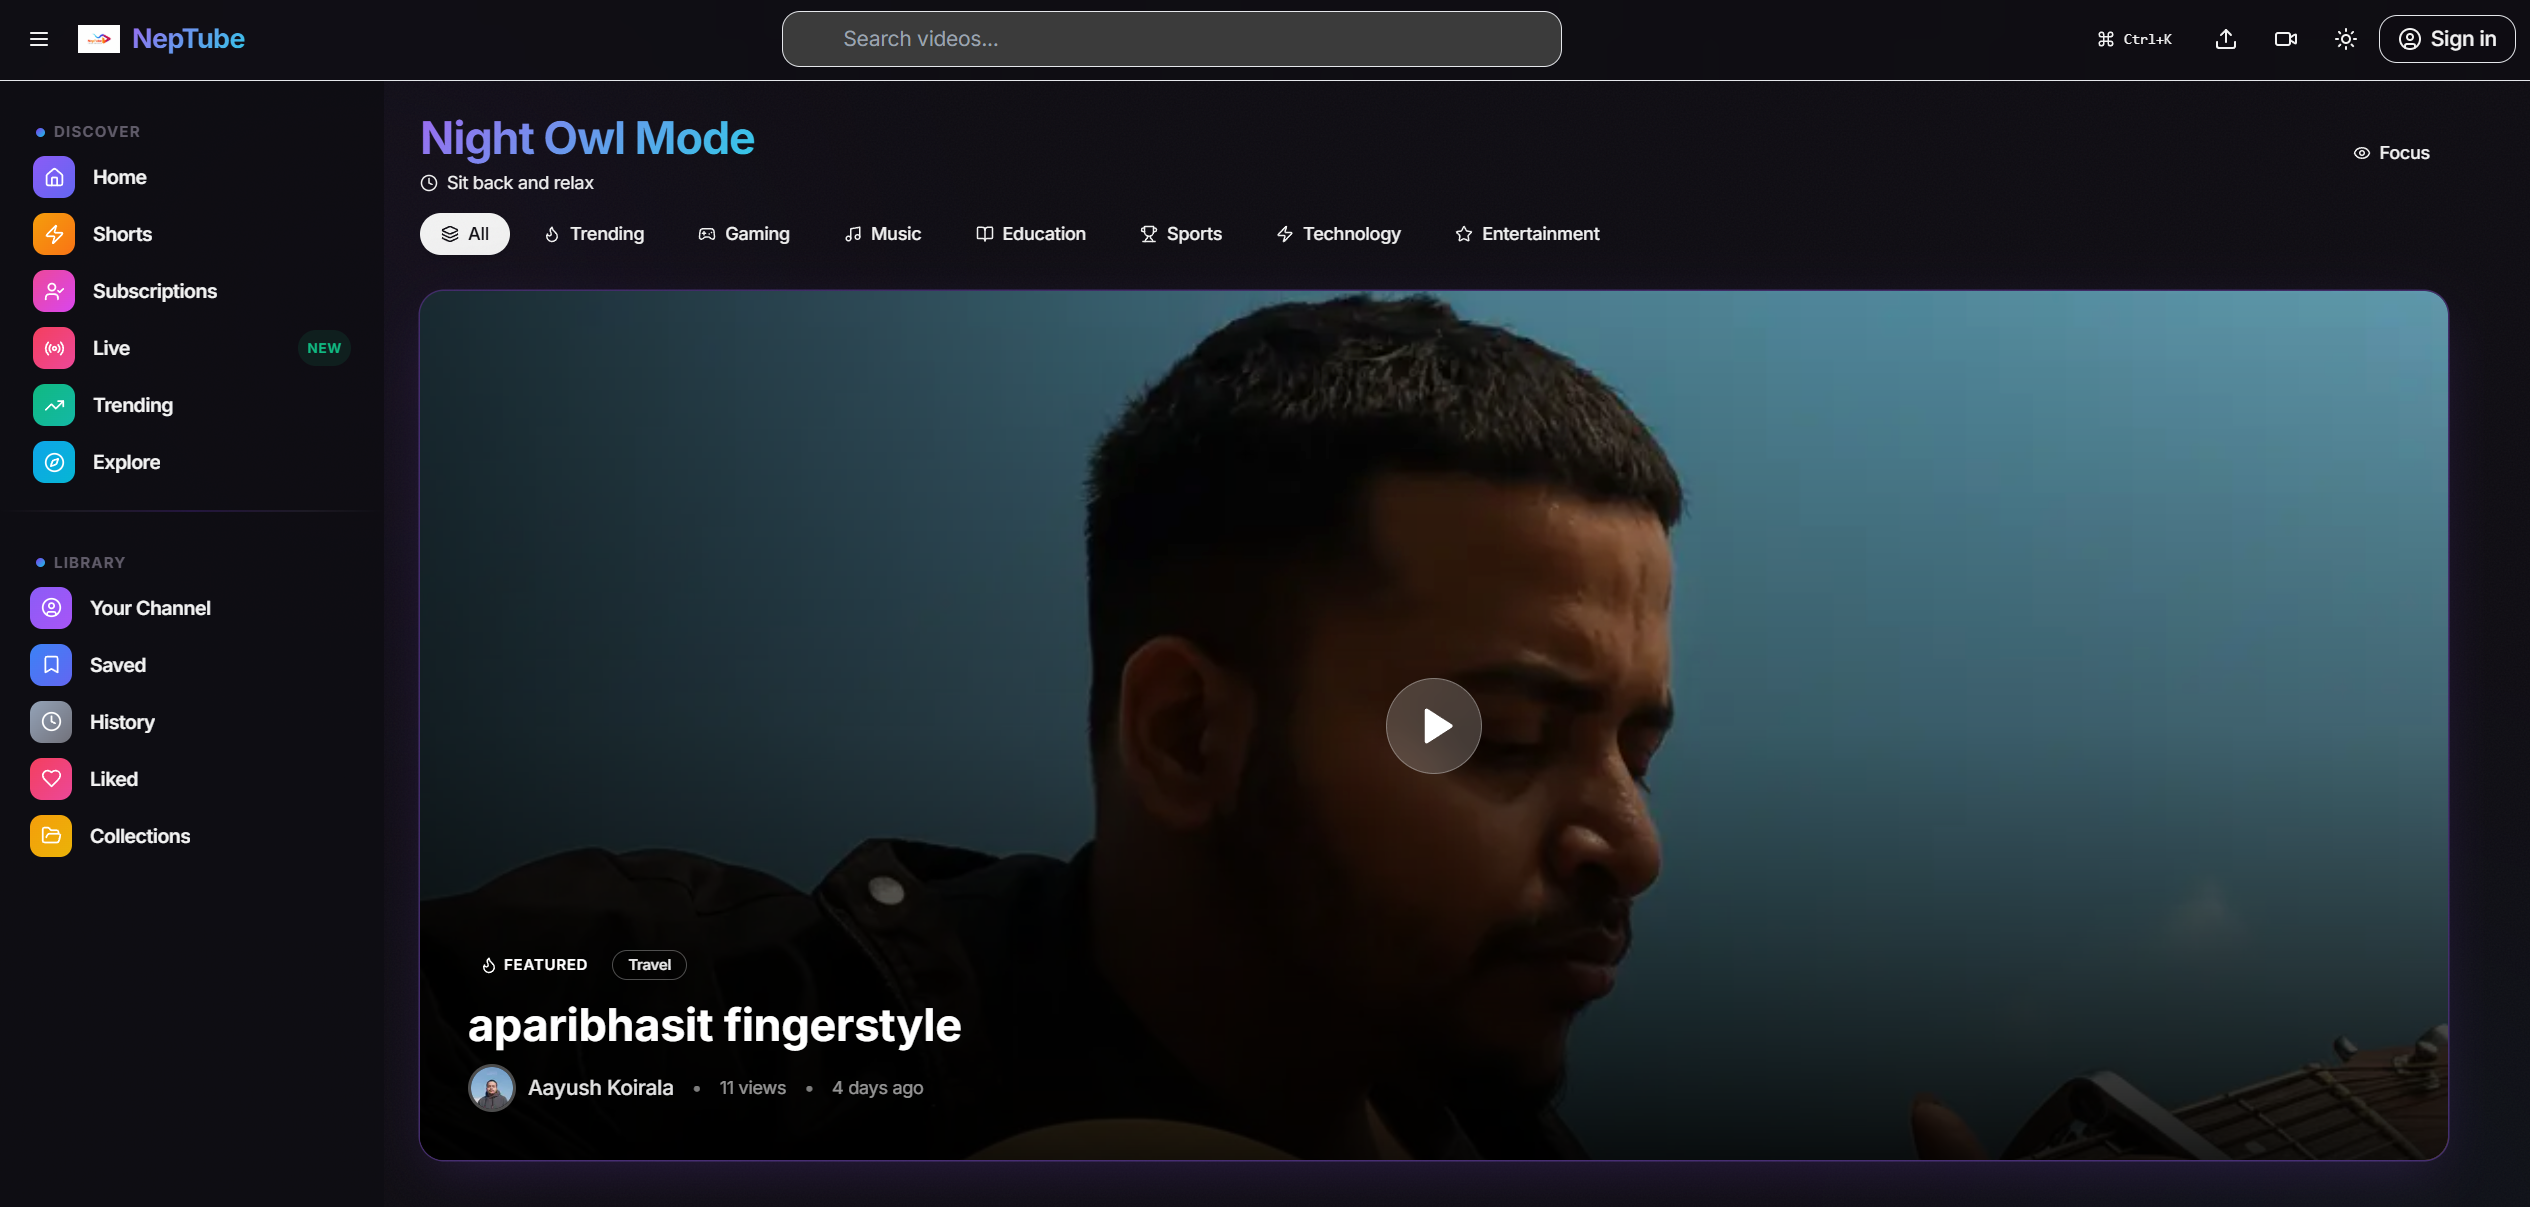
\includegraphics[width=0.80\textwidth,keepaspectratio,max height=0.7\textheight]{images/Homepage.png}
\caption{NepTube Home Page --- Video Browsing Interface}
\label{fig:screenshot-home}
\end{figure}

\subsection{Video Player Interface}

The video player features adaptive bitrate streaming, playback controls, quality selection, and AI-generated subtitles. Users can like, dislike, comment, and add videos to playlists directly from this interface.

\begin{figure}[H]
\centering
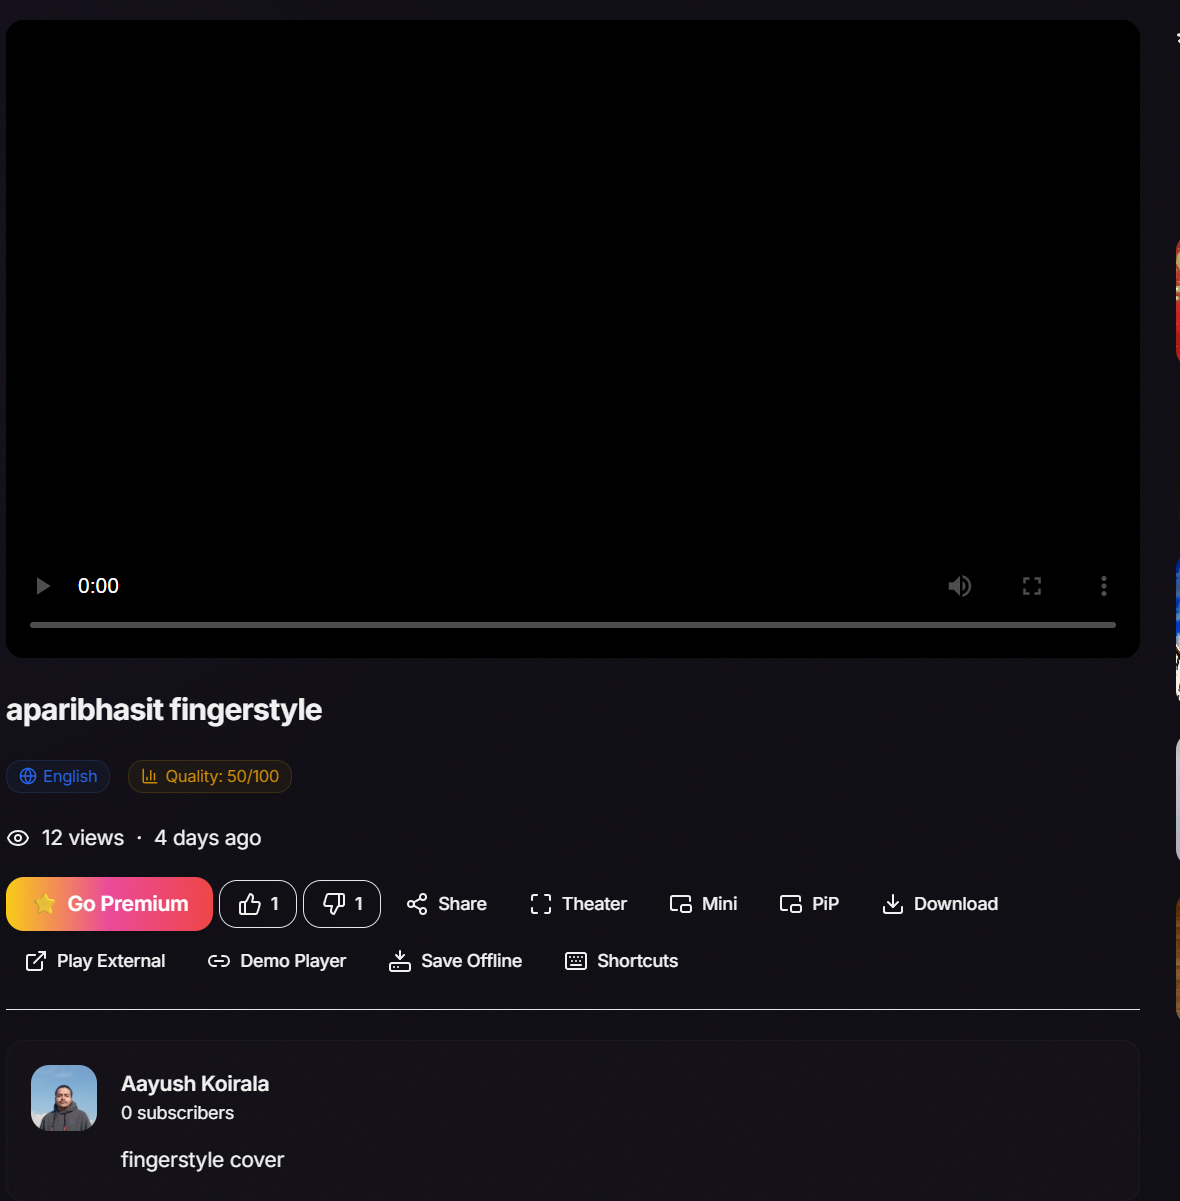
\includegraphics[width=0.80\textwidth,keepaspectratio,max height=0.7\textheight]{images/VideoPlayer.png}
\caption{Video Player with Playback Controls and Social Features}
\label{fig:screenshot-player}
\end{figure}

\subsection{Creator Dashboard}

The creator dashboard provides analytics, video management tools, and AI-powered content optimization features. Creators can upload videos, generate AI thumbnails, view engagement metrics, and manage their channel settings.

\begin{figure}[H]
\centering
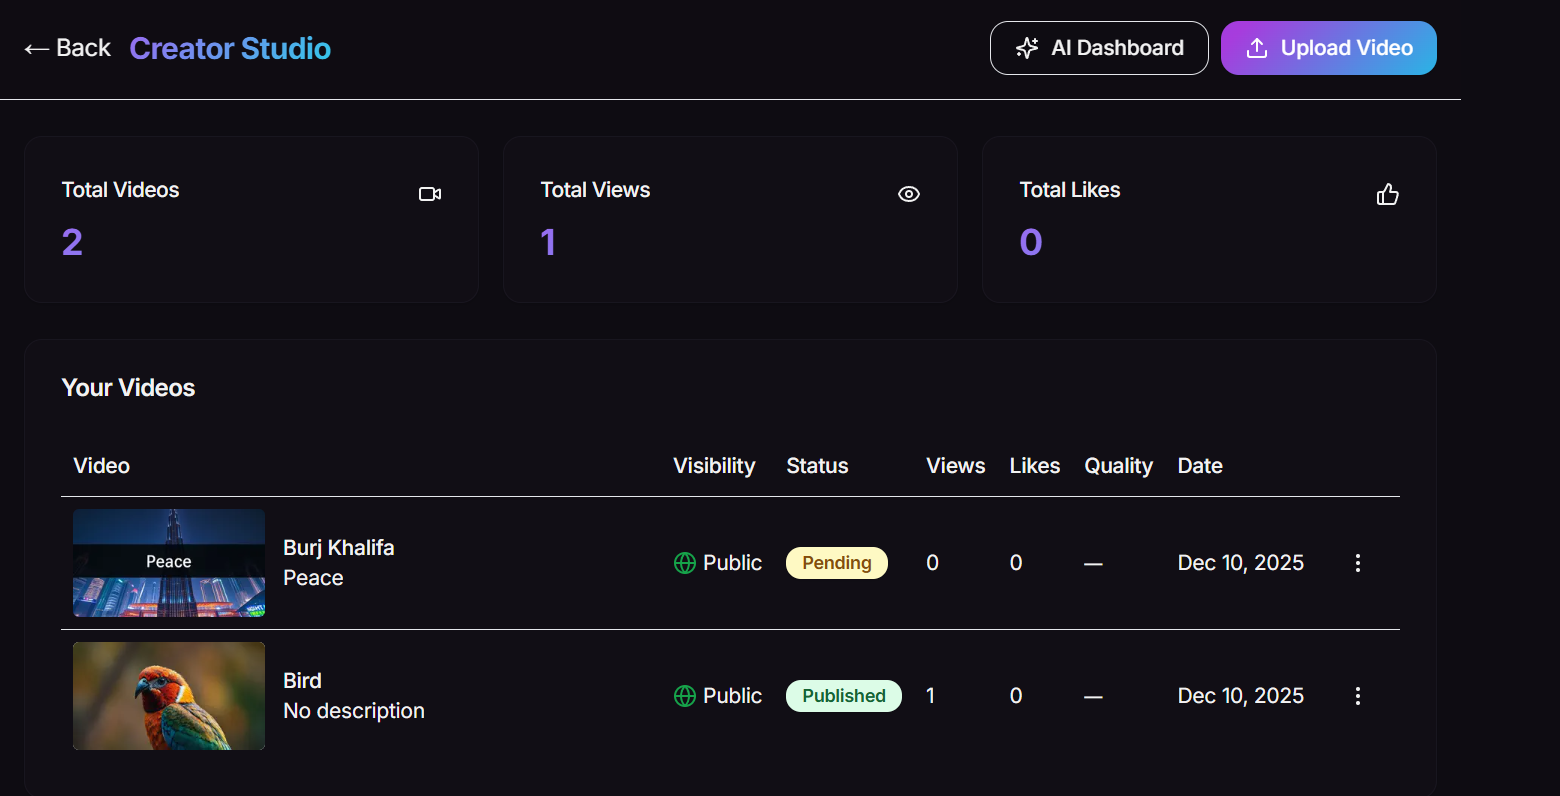
\includegraphics[width=0.80\textwidth,keepaspectratio,max height=0.7\textheight]{images/CreatorDashboard.png}
\caption{Creator Dashboard with Analytics and Video Management}
\label{fig:screenshot-creator}
\end{figure}

\subsection{Admin Dashboard}

The admin dashboard offers comprehensive platform management tools including user management (ban/unban, role changes), content moderation with AI-assisted toxicity detection, report review, and platform analytics.

\begin{figure}[H]
\centering
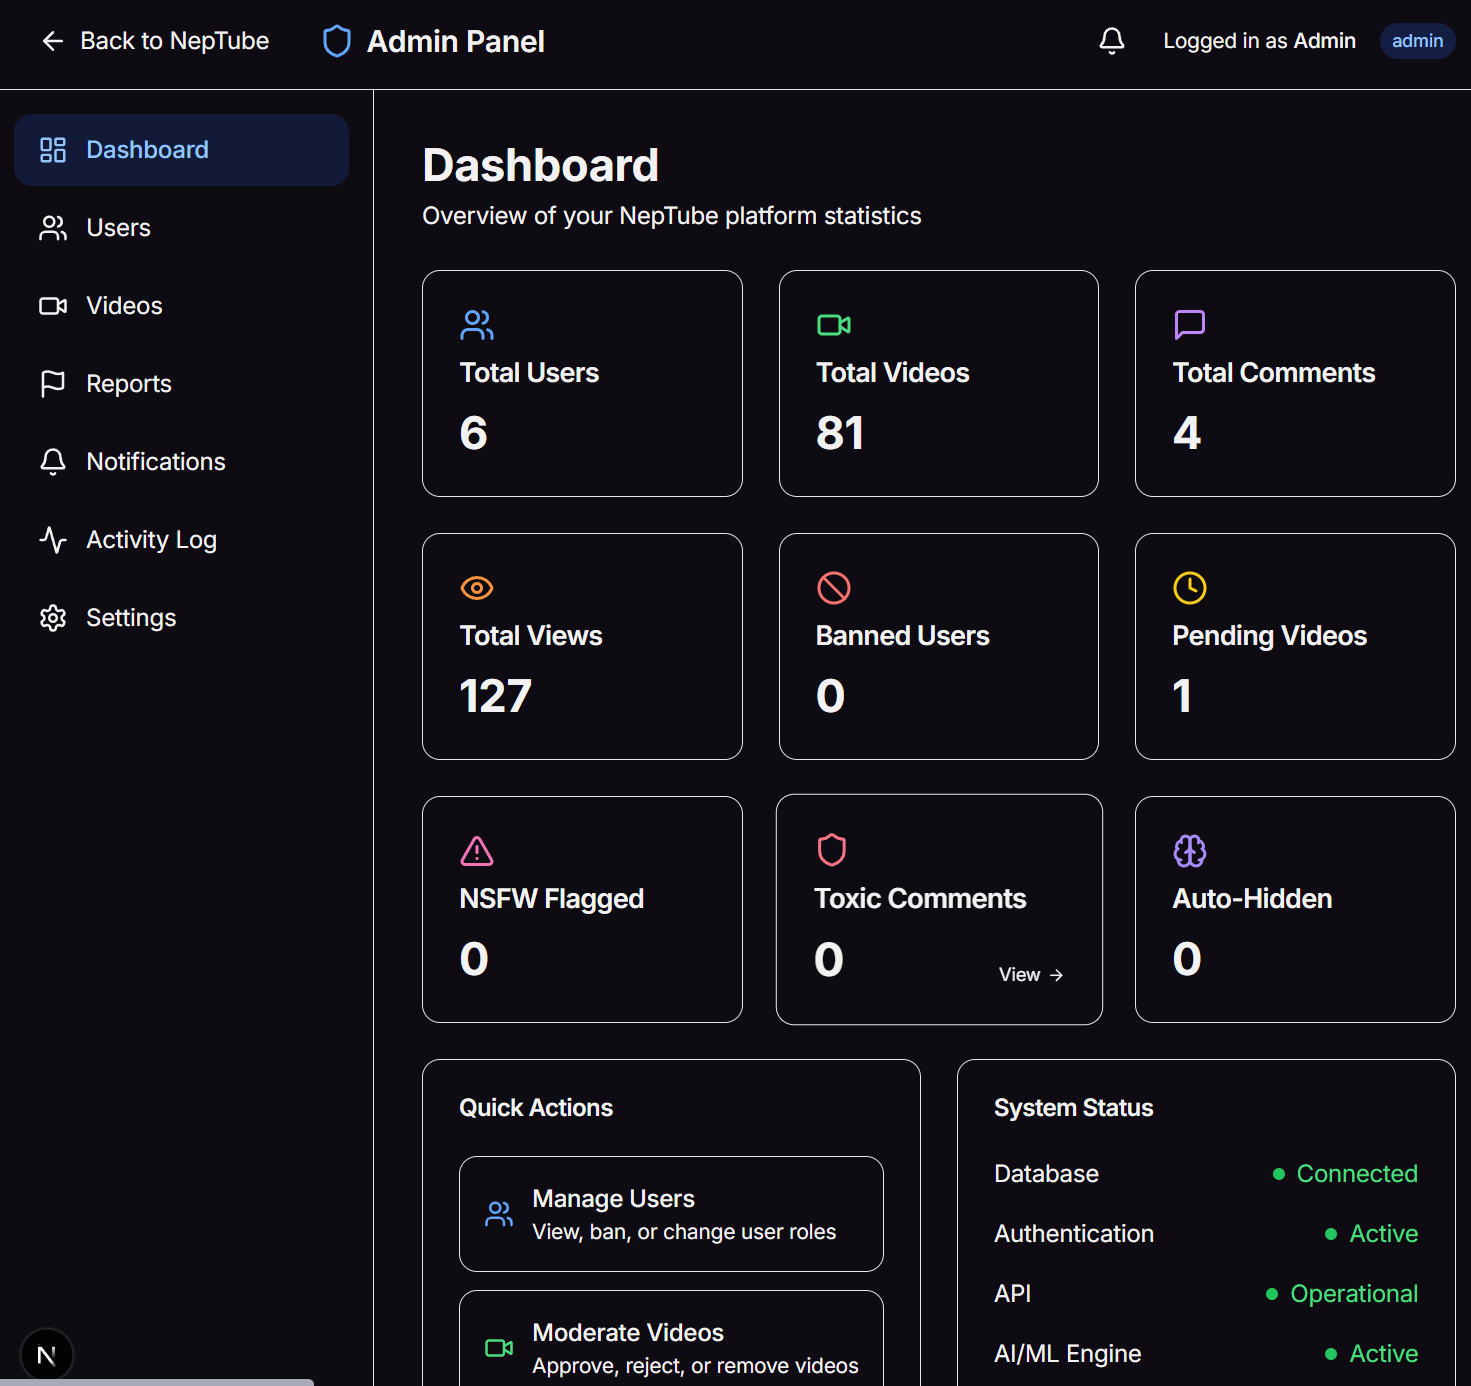
\includegraphics[width=0.80\textwidth,keepaspectratio,max height=0.7\textheight]{images/AdminDashboard.png}
\caption{Admin Dashboard with Moderation and Analytics Tools}
\label{fig:screenshot-admin}
\end{figure}
